\chapter{安装与首次启动}\label{ch:install}
\index{Anzhuang yu Runtime@安装与 Runtime}

KSSOLV Toolbox 可作为独立应用程序运行，也可安装为 MATLAB\regmark{} 工具箱，或在浏览器中使用 \ksonline{}。表\ref{tab:usage-modes}比较了三种方式的运行条件。本章介绍独立应用在 Windows、macOS 和 Linux 上的安装，以及 MATLAB\regmark{} 工具箱的安装与首次启动。

\ksonline{} 无须安装客户端；准备好浏览器与访问地址后，按第\ref{ch:online}章进入工作空间。使用本机应用或 MATLAB\regmark{} 工具箱时，先完成本章对应的安装步骤，再检查界面、导入一个小型结构并保存项目。

\section{确认运行环境}

独立应用由匹配的 MATLAB\regmark{} Runtime 运行，无须完整 MATLAB\regmark{} 及其许可证。Runtime 用来执行应用，不提供桌面编程环境。

MATLAB\regmark{} 工具箱面向已有受支持 MATLAB\regmark{} 及有效许可证的用户。工具箱要求 MATLAB\regmark{} R2025a 或更新版本，安装方法见本章“在 MATLAB\regmark{} 中安装工具箱”一节。已具备 MATLAB\regmark{} 的用户可根据是否需要工作区变量、脚本和其他 MATLAB\regmark{} 产品选择使用方式。

\subsection{认识安装包中的 \headinglatin{Runtime}}

独立应用需要与发行包匹配的 MATLAB\regmark{} Runtime。安装包通常采用三种方式提供运行环境：联网包在需要时下载 Runtime，离线包随附 Runtime，而仅应用包使用计算机上已有的兼容 Runtime。应用版本号和 Runtime 的发行版号含义不同：前者标识 KSSOLV Toolbox，后者标识运行环境。

安装程序会检测独立应用所需的 Runtime。即使已安装完整 MATLAB\regmark{}，仍需按检测结果选择匹配发行版的 Runtime 或继续安装。

\begin{notebox}{选择适合当前计算机的文件}
下载时同时核对操作系统、处理器架构和安装包说明。Apple silicon 与 Intel Mac 使用不同架构的程序；Windows 和 Linux 的程序也不能互换。以发行页提供的文件和说明为准。
\end{notebox}

\section{安装前的准备}

从 KSSOLV Toolbox 项目发行页下载安装文件后，将文件放在容易找到的位置，例如“下载”文件夹。核对发行说明中的版本、操作系统与处理器架构，再选择对应的分发包。

安装前保存项目并关闭旧版 KSSOLV Toolbox。升级通常保留项目和个人设置。联网安装期间保持网络连接；使用离线包时，将全部随附文件放在同一目录。

安装位置可选择有足够空间的本地磁盘。应用、Runtime 与个人项目可以放在不同目录：前两者由安装器管理，项目则建议集中放在一个自己熟悉的文件夹中。例如建立“材料计算”文件夹，再按材料或项目分别建立子文件夹。这样的安排比把所有项目留在下载目录更便于查找。


\section{在 \headinglatin{Windows} 上安装}

\subsection{运行安装程序}

Windows 的独立分发包通常是带有版本号的 EXE 安装程序，文件名中包含 \file{KSSOLV_Toolbox} 和发行版本。部分离线包包含同名的 \file{.bin} 分卷文件。遇到这种形式时，把这些文件放在同一文件夹，再运行 EXE；不需要手动打开分卷。

\begin{steps}
\item 双击安装程序。若系统显示用户账户控制窗口，确认程序来源后允许继续。
\item 选择安装语言并阅读安装说明。简体中文安装界面适合与本手册对照使用。
\item 按页面要求确认工具箱和 Runtime 的许可，并继续到安装位置与 Runtime 设置。
\item 选择应用目录。可以保留默认位置，也可以选择另一块本地磁盘。
\item 检查 Runtime 的检测结果：已有兼容环境时按提示复用；没有时选择安装包提供的安装方式。
\item 点击安装，等待文件复制和最后的配置完成。显示完成页面后退出安装器。
\end{steps}

应用和 Runtime 的位置可以分别选择，例如：
\begin{itemize}[nosep]
\item 应用目录：\literalinput{E:/Apps/KSSOLV Toolbox}。
\item Runtime 目录：\literalinput{E:/MathWorks/MATLAB Runtime}。
\end{itemize}
Runtime 目录需使用 ASCII 字符，可使用英文、数字和空格；项目名称则可以按照自己的研究内容命名。


\subsection{等待安装完成}

安装程序在最后阶段完成运行环境配置。首次安装 Runtime 时，这一阶段可能较慢，等待安装器显示完成即可。

如果配置未完成，按提示重试，并检查磁盘空间、目录权限和 Runtime 来源。

默认安装供所有用户使用，通常需要管理员授权。个人安装与已有 Runtime 的复用方式取决于分发包提供的选项。普通安装无需修改系统 PATH，也无需到 MATLAB\regmark{} 目录手动复制库文件。

\subsection{启动与更新}

完成安装后，从开始菜单或安装器创建的快捷方式启动 KSSOLV Toolbox。启动卡片会显示产品名称和当前启动状态；主窗口出现后，再等待项目面板和工具栏完成显示。

更新时运行新的安装包，按照向导替换旧版应用。已登记的旧版由安装器处理，共享 Runtime、个人配置和项目通常保留。应用安装目录不应当作为个人项目目录，后续升级时也更容易分清程序文件与自己的数据。

\begin{notebox}{离线包的检查点}
如果安装器提示找不到附加文件，先检查 EXE 和全部同名分卷是否在一起，文件名是否被浏览器自动增加了重复编号。确认下载完整后，再重新运行安装程序。
\end{notebox}

\section{在 macOS 上安装}

\subsection{选择与 \headinglatin{Mac} 匹配的分发包}

在苹果菜单的“关于本机”中可以查看处理器信息。Apple silicon 安装包面向采用 Apple 芯片的 Mac，选择分发包时应核对所需架构。

macOS 使用原生安装器完成 PKG 安装。应用通常放在 \file{/Applications}，安装器会检测所需的 Runtime，并根据安装包类型复用、下载或安装运行环境。整个过程在系统安装向导中完成。

安装向导的介绍页列出应用版本、处理器架构和 MATLAB\regmark{} Runtime 要求。开始安装前，核对这些信息是否与当前 Mac 匹配，并确认安装包是仅包含应用，还是同时提供运行环境；具体要求以所用安装包的介绍页为准。

\begin{steps}
\item 打开下载的分发文件，运行其中的 PKG 安装包。
\item 阅读介绍页，确认应用版本、处理器架构和 Runtime 发行版。
\item 按向导阅读并确认许可，然后进入安装类型与位置设置。
\item 选中 KSSOLV Toolbox，检查应用的安装位置；通常保留“应用程序”目录即可。
\item 检查 Runtime 设置，按下一小节说明选择已有环境或由安装器准备环境。
\item 开始安装，并在系统要求时完成管理员认证。
\item 等待安装程序报告成功，再从“应用程序”打开 KSSOLV Toolbox。
\end{steps}

许可页如图~\ref{fig:install-macos-license}~所示。可直接阅读条款，也可使用窗口下方的 \ui{打印…} 或 \ui{保存…} 留存文本。阅读后点击 \ui{继续}，按随后出现的对话框确认是否同意；同意后才能进入后续安装步骤。向导最后显示成功页面后，安装才告完成。

\screenshot{publication-assets/crop-b9b8c6192e335985ecb0.png}{macOS 安装向导的许可页。可在窗口中阅读条款，也可打印或保存许可文本。}{fig:install-macos-license}


\subsection{处理已有的 \headinglatin{Runtime}}

如果使用仅应用安装包，计算机上必须已经具备兼容的 Runtime。自动检测不到时，在安装类型页选中“已有 MATLAB\regmark{} Runtime”，通过“位置”进入“其他…”，选择安装器所要求的发行版文件夹。应选择 Runtime 的根目录，而不是它内部某个库目录。

联网安装包会在缺少 Runtime 时从 MathWorks 下载；离线包则使用随包提供的内容。已有环境的发行版、架构和所需组件符合要求时可以复用。安装器完成 Runtime 准备后，再替换旧版工具箱。

安装最后阶段会在后台完成配置，不一定出现 Toolbox 主窗口。待系统安装器显示成功后，再主动启动应用。第一次打开时出现启动卡片属于正常过程；后续每次启动仍需要加载运行环境，只是无需重复进行安装。

\subsection{保留项目并升级}

升级前先保存并关闭应用，再运行新安装包。共享 Runtime、用户配置和项目不需要因为更换 Toolbox 而逐一移走。建议把 \file{.ks} 文件放在自己的“文稿”或课题目录，而不是应用包内部。

如果系统询问是否允许打开从互联网下载的应用，按 macOS 显示的来源信息完成确认。

\section{在 \headinglatin{Linux} 上安装}

Linux 独立应用应使用对应平台的安装文件，并在图形桌面会话中运行。下载完成后，若文件已经可以直接执行，可以从文件管理器启动；如果没有执行权限，可在文件所在目录打开终端。

\begin{steps}
\item 在终端进入安装文件所在目录。
\item 为安装文件增加执行权限：\texttt{chmod +x KSSOLV\_Toolbox.install}。
\item 运行 \texttt{./KSSOLV\_Toolbox.install}，进入图形安装向导。
\item 按向导选择应用和 Runtime 位置，等待安装完成。
\item 按安装完成页提供的入口或启动命令启动应用。
\end{steps}

这里的文件名用于说明常见形式，具体名称以下载内容为准。安装程序最后显示的 Runtime 路径与启动命令应保存下来，尤其是在没有自动创建应用菜单项的桌面环境中。

Linux 独立应用需要图形桌面会话；使用 \ksonline{} 时，直接在浏览器中打开在线版入口即可。


\section{在 \headinglatin{MATLAB}\regmark{} 中安装工具箱}

已有完整 MATLAB\regmark{} 的读者可以使用 \file{KSSOLV_Toolbox.mltbx}。开始前，在 MATLAB\regmark{} 中确认版本达到 R2025a 或更新版本，然后完成以下操作。

\begin{steps}
\item 从项目发行页下载 \file{KSSOLV_Toolbox.mltbx}。
\item 在 MATLAB\regmark{} 中打开该文件，按附加功能安装窗口完成安装。
\item 从 MATLAB\regmark{} 或附加功能管理器启动 KSSOLV Toolbox。
\item 确认主窗口出现，再进行项目练习。
\end{steps}

如果计算机上已有其他版本，使用 MATLAB\regmark{} 的附加功能管理器查看和管理已安装的工具箱。安装或升级后，确认 MATLAB\regmark{} 与工具箱版本兼容，再继续已有项目。

本手册以图形界面为主，通用的结构导入、建模和工作流步骤适用于三种使用方式。涉及本机文件、云端目录、MATLAB\regmark{} 工作区或额外 MATLAB\regmark{} 产品时，正文分别说明对应操作与所需环境。

\section{第一次启动后的练习}

打开独立应用程序时，会先出现启动卡片。图~\ref{fig:desktop-startup-050}~中的卡片显示产品版本与当前加载状态，此时应用正在准备工作区。首次启动或更新后，加载运行环境可能需要较长时间；保留启动窗口，等待主窗口出现。

\begin{figure}[!htb]
\centering
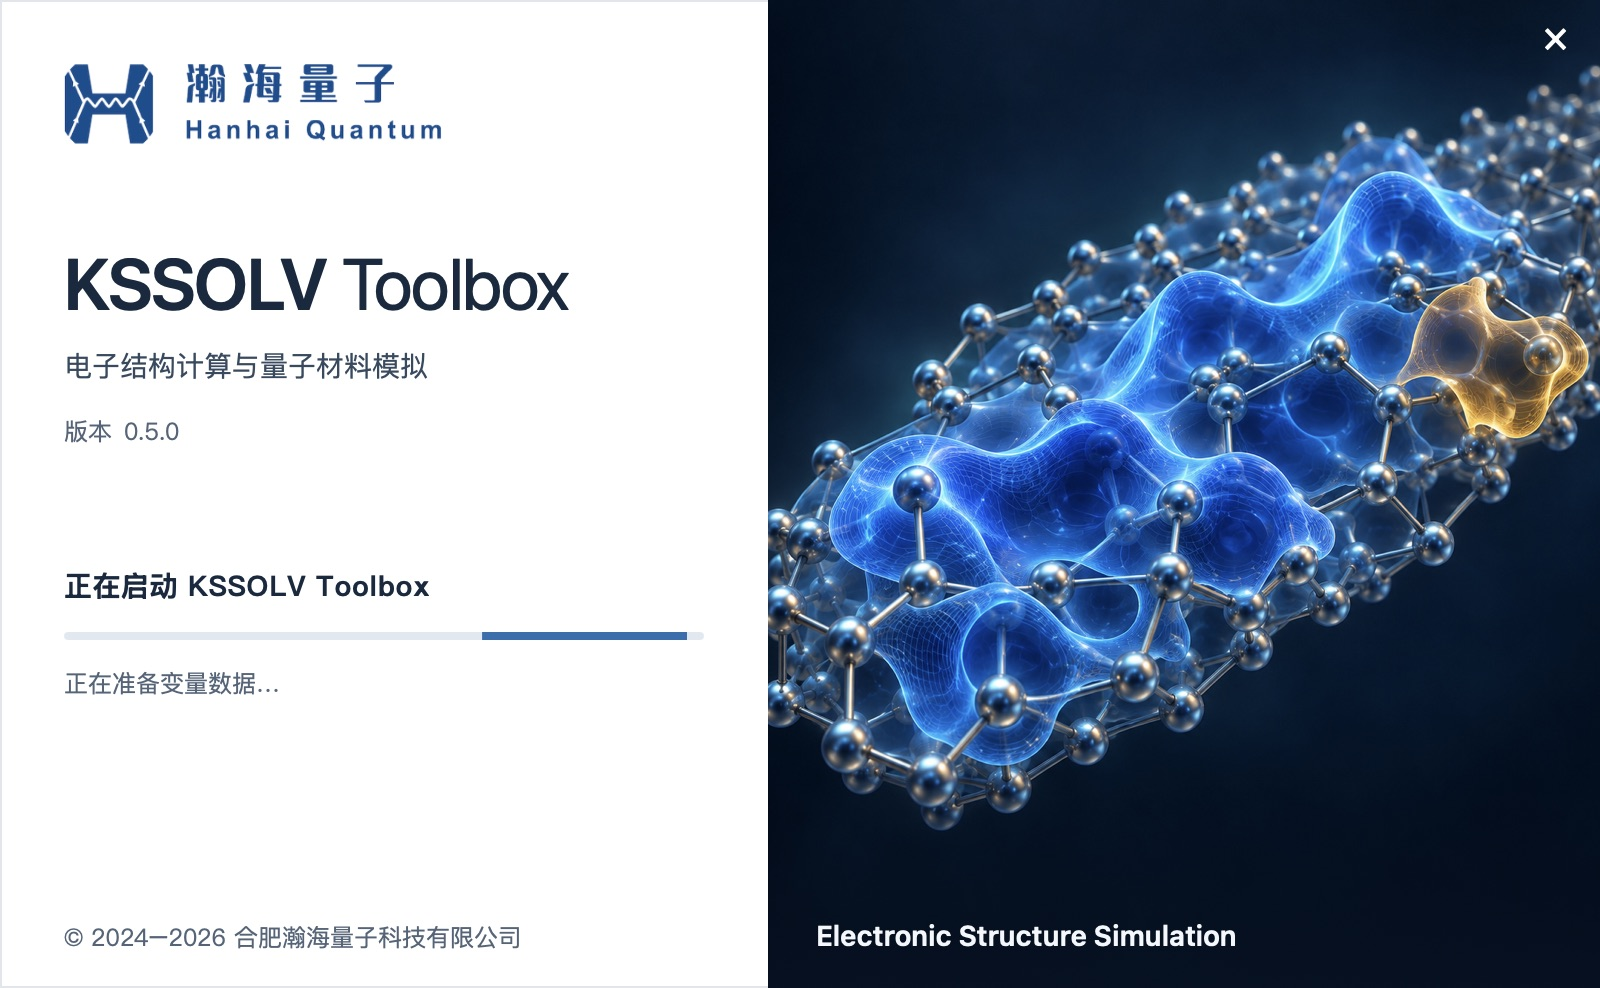
\includegraphics[width=122mm]{publication-assets/crop-6bf7d3c41caf0892911f.png}
\caption{KSSOLV Toolbox V0.5.0 独立应用的启动卡片，显示产品版本与加载状态。}
\label{fig:desktop-startup-050}
\end{figure}

启动卡片收起后，主窗口显示项目浏览器、功能区和中央文档区，可以开始下面的版本检查与项目练习。

\subsection{确认界面和版本}

主窗口出现后，先找到上方的\ui{主页}功能区和左侧\ui{项目浏览器}，再选择\ui{主页 → 帮助 → 关于 KSSOLV}核对产品版本。本书适用版本为 V0.5.0。界面语言在\ui{主页 → 设置 → 通用}中选择，修改后下次启动生效。

图\ref{fig:install-workspace-overview}展示空项目中展开主要面板后的完整界面。上方功能区用于导入结构、建立工作流和运行任务；左侧项目浏览器列出工作内容，下方信息浏览器显示所选对象的属性。中央文档区显示欢迎文字，导入结构后会出现三维视图；右侧配置编辑器填写参数，模拟浏览器显示运行输出。底部命令行窗口提供交互命令入口，图形教程不要求在这里输入命令。

\begin{figure}[!htb]
\centering
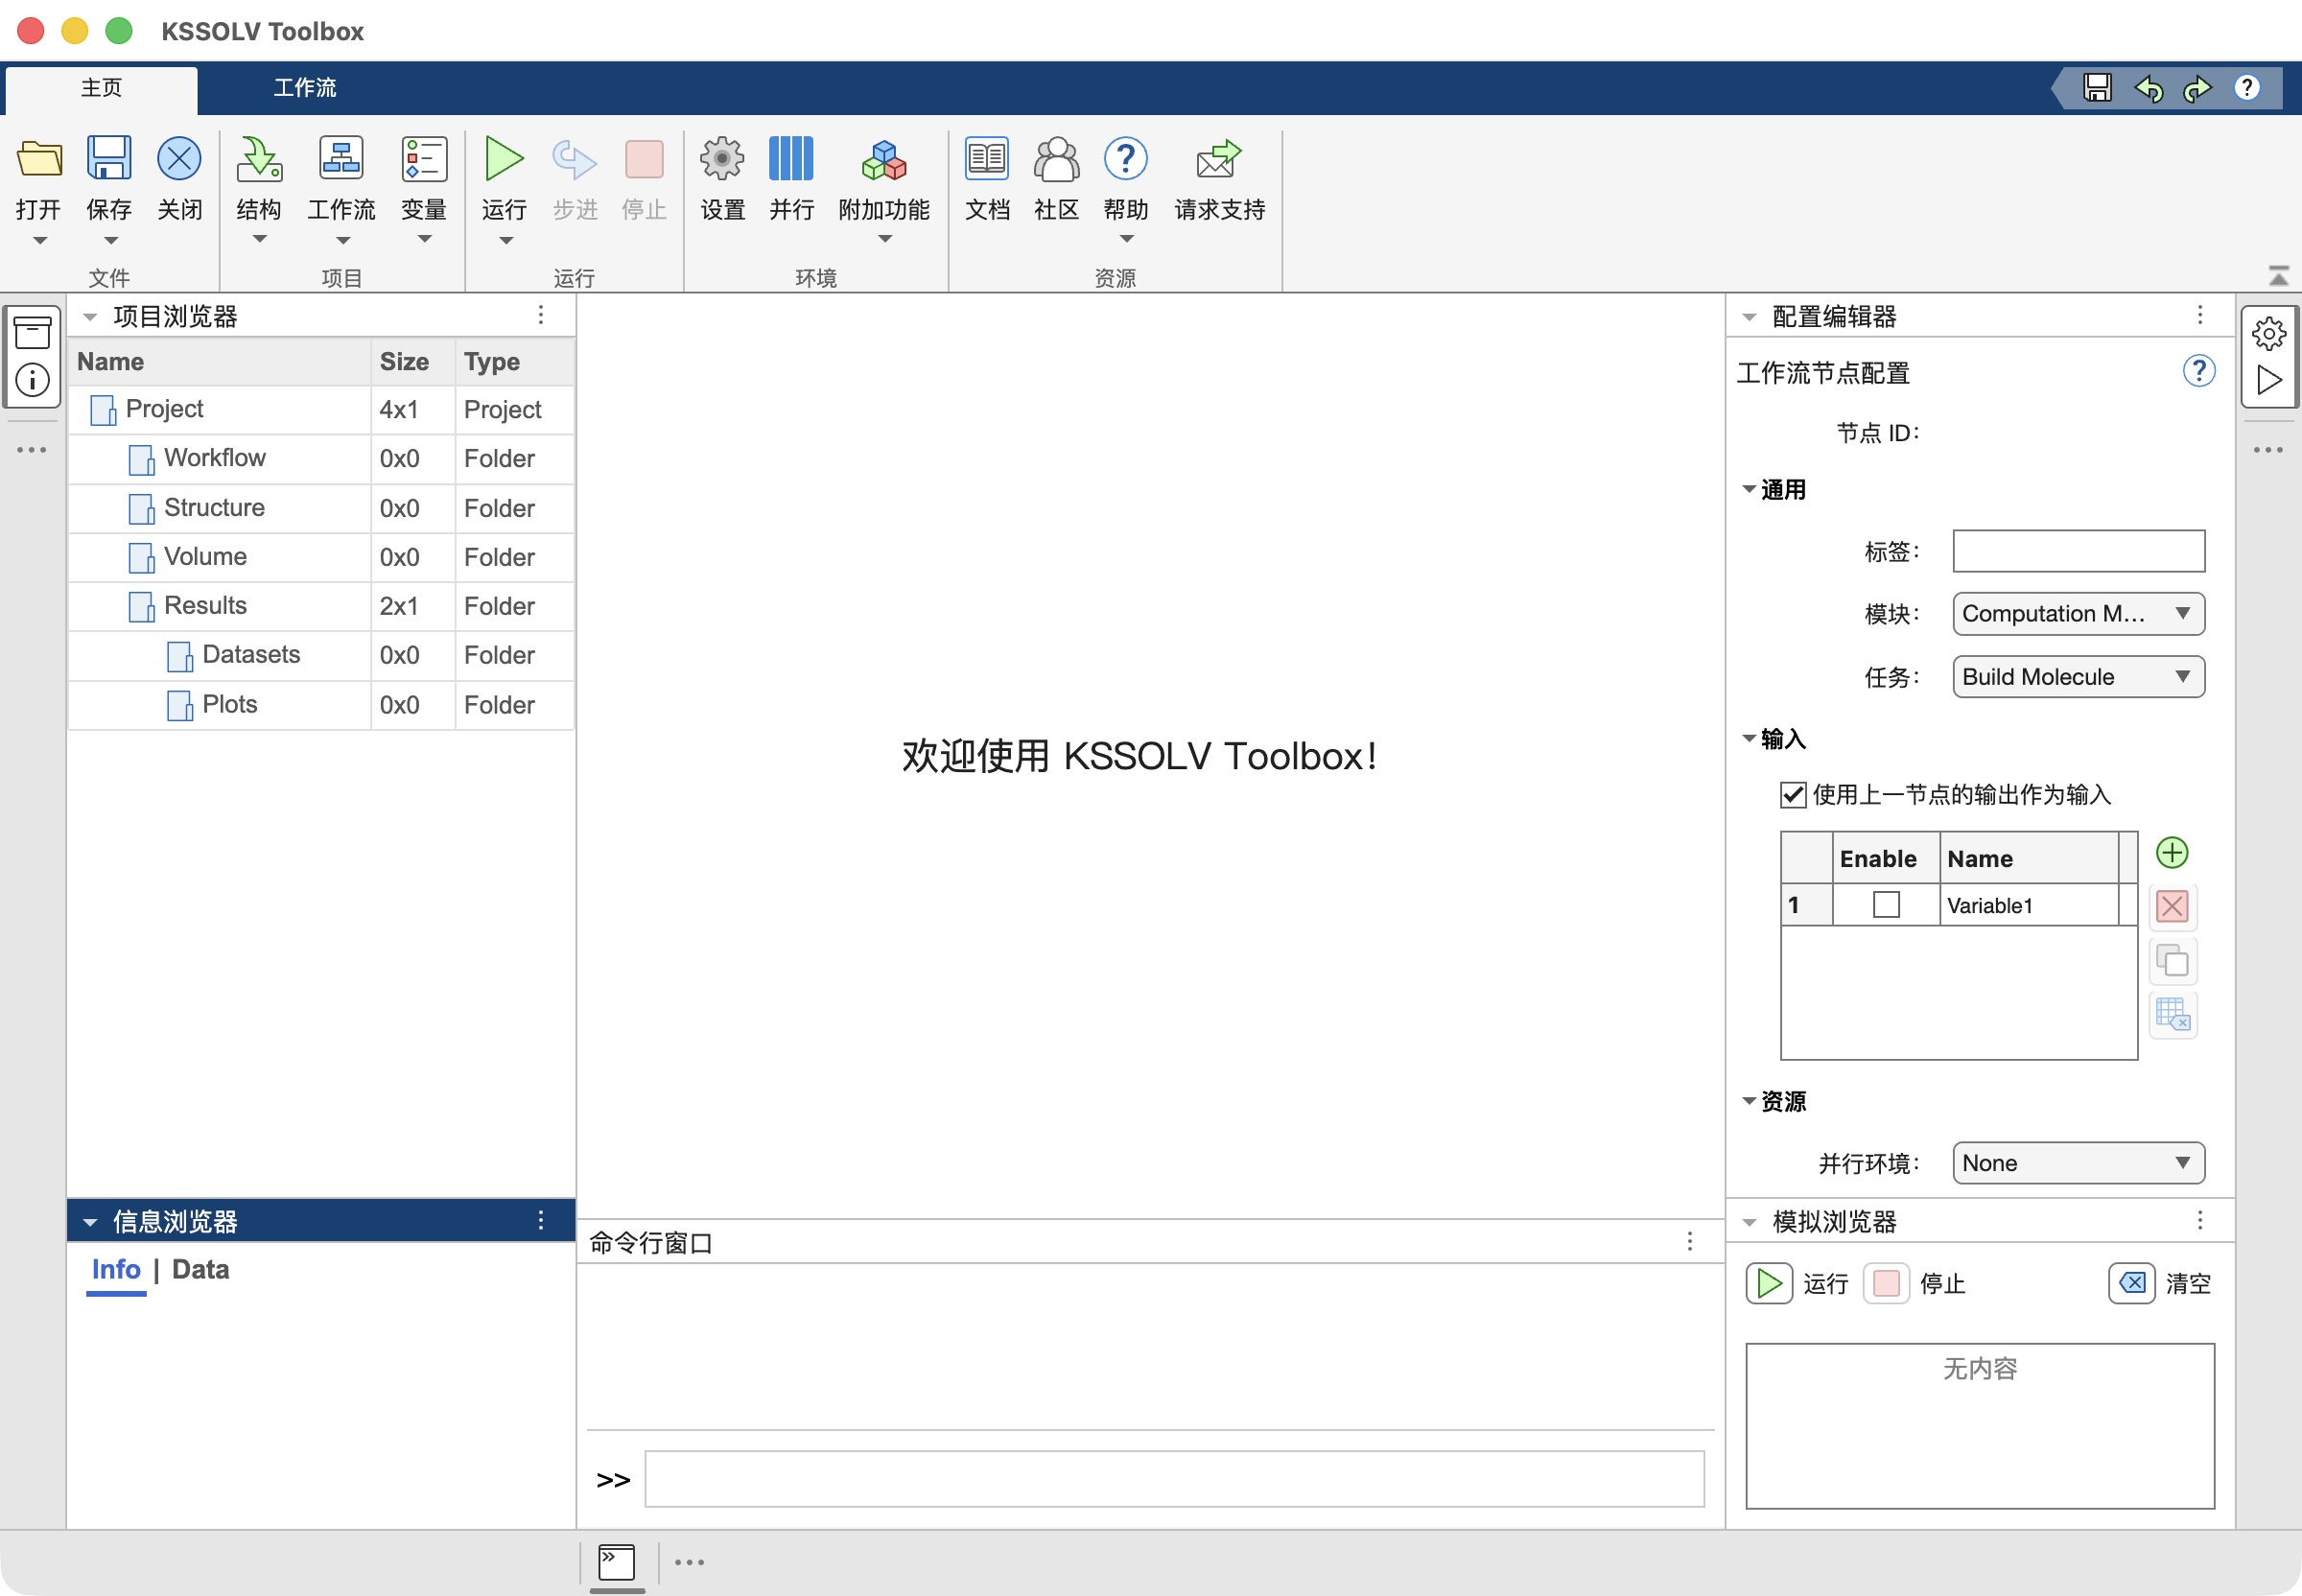
\includegraphics[width=\linewidth]{publication-assets/crop-c885d8ed3b1bcd221501.png}
\caption{独立应用程序的完整工作区布局。项目、信息、配置、模拟和命令行面板均已展开；中央尚未打开结构或工作流文档。}
\label{fig:install-workspace-overview}
\end{figure}

首次进入时，部分面板处于收起状态。可以通过左右侧边按钮组展开相应区域，或从省略号的\ui{打开面板}列表选择需要的面板。首次练习主要使用结构导入与项目保存入口；各区域的具体用法见第\ref{ch:workspace}章。

\subsection{创建一个可以重新打开的项目}

这项练习只检查文件与界面，不需要运行计算。准备随书的 \file{examples/silicon.cif}，也可使用自己的小型 CIF、XYZ 结构文件。使用随书硅结构时，可直接与第\ref{ch:workspace}章的工作区练习衔接。

\begin{steps}
\item 选择 \ui{主页 → 结构 → 从文件导入结构…}，选中准备好的结构文件。
\item 确认结构名称出现在项目浏览器中，中央三维视图显示原子。
\item 用鼠标拖动旋转视图，再用滚轮调整大小，确认结构能够完整显示。
\item 点击 \ui{保存}，在自己的工作目录输入 \file{first-project.ks}。
\item 确认保存完成后关闭当前项目，再通过 \ui{打开项目…} 打开刚保存的文件。
\item 检查项目浏览器和结构文档，确认此前导入的结构仍在。
\end{steps}


完成这项练习后，即可使用结构导入、三维显示和项目保存功能。第一次电子结构计算见第~\ref{ch:first}~章。

\section{遇到问题时先检查什么}

如果程序未能启动，检查安装包是否匹配处理器架构，Runtime 是否为安装器要求的版本。需要反馈问题时，提供 Toolbox 版本、操作系统、安装位置和窗口中的完整提示。

如果主窗口出现但三维结构没有显示，先用本章的小结构重试，并观察是否有明确的图形提示。在线版还需使用能运行 WebGL 的浏览器。若文件导入后没有新增项目项，核对结构文件格式和内容。

如果保存时找不到文件，先确认保存位置：独立应用与 MATLAB\regmark{} 工具箱使用本机目录，\ksonline{} 使用服务器上的工作目录。云端“文件”面板的操作，以及上传与下载练习，见第\ref{ch:online}章。

\subsection{为后续练习整理文件}

为项目建立固定目录，分别保存原始结构和工作项目，保留原始文件的来源与名称。在结构准备、参数检查和结果整理完成时另存项目副本，便于回到已有阶段。跨计算机传递时优先使用完整的 \file{.ks} 项目；单独的结构文件通常不包含工作流和计算结果。

